\documentclass[\string~/GitHub/sthlmNordBeamerTheme/sthlmNordLightDemo.tex]{subfiles}

\begin{document}
%=-=-=-=-=-=-=-=-=-=-=-=-=-=-=-=-=-=-=-=-=-=-=-=-=-=-=-=-=-=-=-=-=-=-=-=-=-=-=-=
%   FRAME START   -=-=-=-=-=-=-=-=-=-=-=-=-=-=-=-=-=-=-=-=-=-=-=-=-=-=-=-=-=-=-=
\begin{frame}[allowframebreaks, allowdisplaybreaks, t]{Example}{Completing The Square}

	\prob Solve the equation \( x^2 + 2x - 3 = 0 \) by completing the square.

	\mref{ma2c-5000-2022-Q2119a\cite{alfredssonMatematik5000Kurs2021}\index{ma2c-5000-2022-2000!Q2119a}}

	\framebreak
	\soln \hfill\\
	\begin{minipage}[t]{0.5\textwidth}
		\vspace{0pt}
		\begin{align*}
			x^2 + 2x - 3                                   & = 0 \\
			x^2 + 2x + \oneg 3                             & = 0 \\
			x^2 + 2x + \cRed{k} + \cRed{\oneg k} + \oneg 3 & = 0
		\end{align*}
	\end{minipage}
	\hspace{0.05\textwidth}
	\begin{minipage}[t]{0.4\textwidth}
		\vspace{0pt}
		\begin{center}
			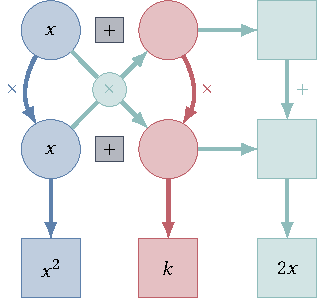
\includegraphics[width=0.8\textwidth]{imgs.tikz.057w}
		\end{center}
	\end{minipage}
	\hfill

	\framebreak

	\hfill\\
	\begin{minipage}[t]{0.5\textwidth}
		\vspace{0pt}
		\begin{align*}
			x^2 + 2x + \cRed{k} + \cRed{\oneg k} + \oneg 3 & = 0        \\
			x^2 + 2x + \cRed{1} + \cRed{\oneg 1} + \oneg 3 & = 0        \\
			(x + 1)^2 + \oneg 4                            & = 0        \\
			(x + 1)^2                                      & = 4        \\
			\sqrt{(x + 1)^2}                               & = \sqrt{4} \\
			\abs{x + 1}                                    & = 2
		\end{align*}
		Now we can consider both cases of \( \abs{x + 1} \).
	\end{minipage}
	\hspace{0.05\textwidth}
	\begin{minipage}[t]{0.4\textwidth}
		\vspace{0pt}
		\begin{center}
			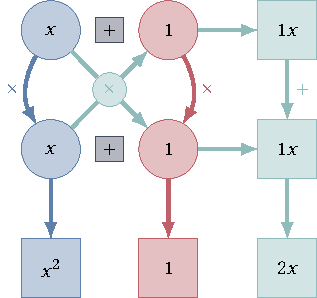
\includegraphics[width=0.8\textwidth]{imgs.tikz.057x}
		\end{center}
	\end{minipage}
	\hfill

	\framebreak

	\hfill\\
	\begin{minipage}[t]{0.45\textwidth}
		\vspace{0pt}
		\textbf{Case I: Positive Case}
		\begin{align*}
			x + 1 & = 2           \\
			x     & = \oneg 1 + 2 \\
			      & = 1
		\end{align*}
	\end{minipage}
	\hspace{0.05\textwidth}
	\begin{minipage}[t]{0.45\textwidth}
		\vspace{0pt}
		\textbf{Case II: Negative Case}
		\begin{align*}
			-(x + 1) & = 2                 \\
			x + 1    & = \oneg 2           \\
			x        & = \oneg 1 + \oneg 2 \\
			         & = \oneg 3
		\end{align*}

	\end{minipage}
	\hfill
\end{frame}
%   FRAME END   --==-=-=-=-=-=-=-=-=-=-=-=-=-=-=-=-=-=-=-=-=-=-=-=-=-=-=-=-=-=-=
%=-=-=-=-=-=-=-=-=-=-=-=-=-=-=-=-=-=-=-=-=-=-=-=-=-=-=-=-=-=-=-=-=-=-=-=-=-=-=-=
\end{document}